The objective of the design of cloud deployments is to achieve cloud agnosticism, which implies that it can operate seamlessly with any cloud provider with minimal or no modifications. To achieve this, all services are intended to be deployed within a Kubernetes cluster, regardless of the location or configuration of the cluster. This is feasible as most major cloud providers offer Kubernetes as a Service (KaaS), and it is also widely available among smaller providers.

The comprehensive design of the cloud services is depicted in Figure \ref{fig:cloud_services}. The communication between the various services is established in two ways:
\begin{itemize}
    \item Through the Cloud Broker: The backend and cloud-Agent services are both subscribers to a set of topics and exchange information through MQTT messages sent to the Cloud Broker.
    \item Through REST Endpoints: The backend services expose REST endpoints which are consumed by the frontend. The frontend is designed to solely serve HTML documents and function as a consumer of the backend endpoints.
\end{itemize}

\begin{figure}[H]
    \centering
    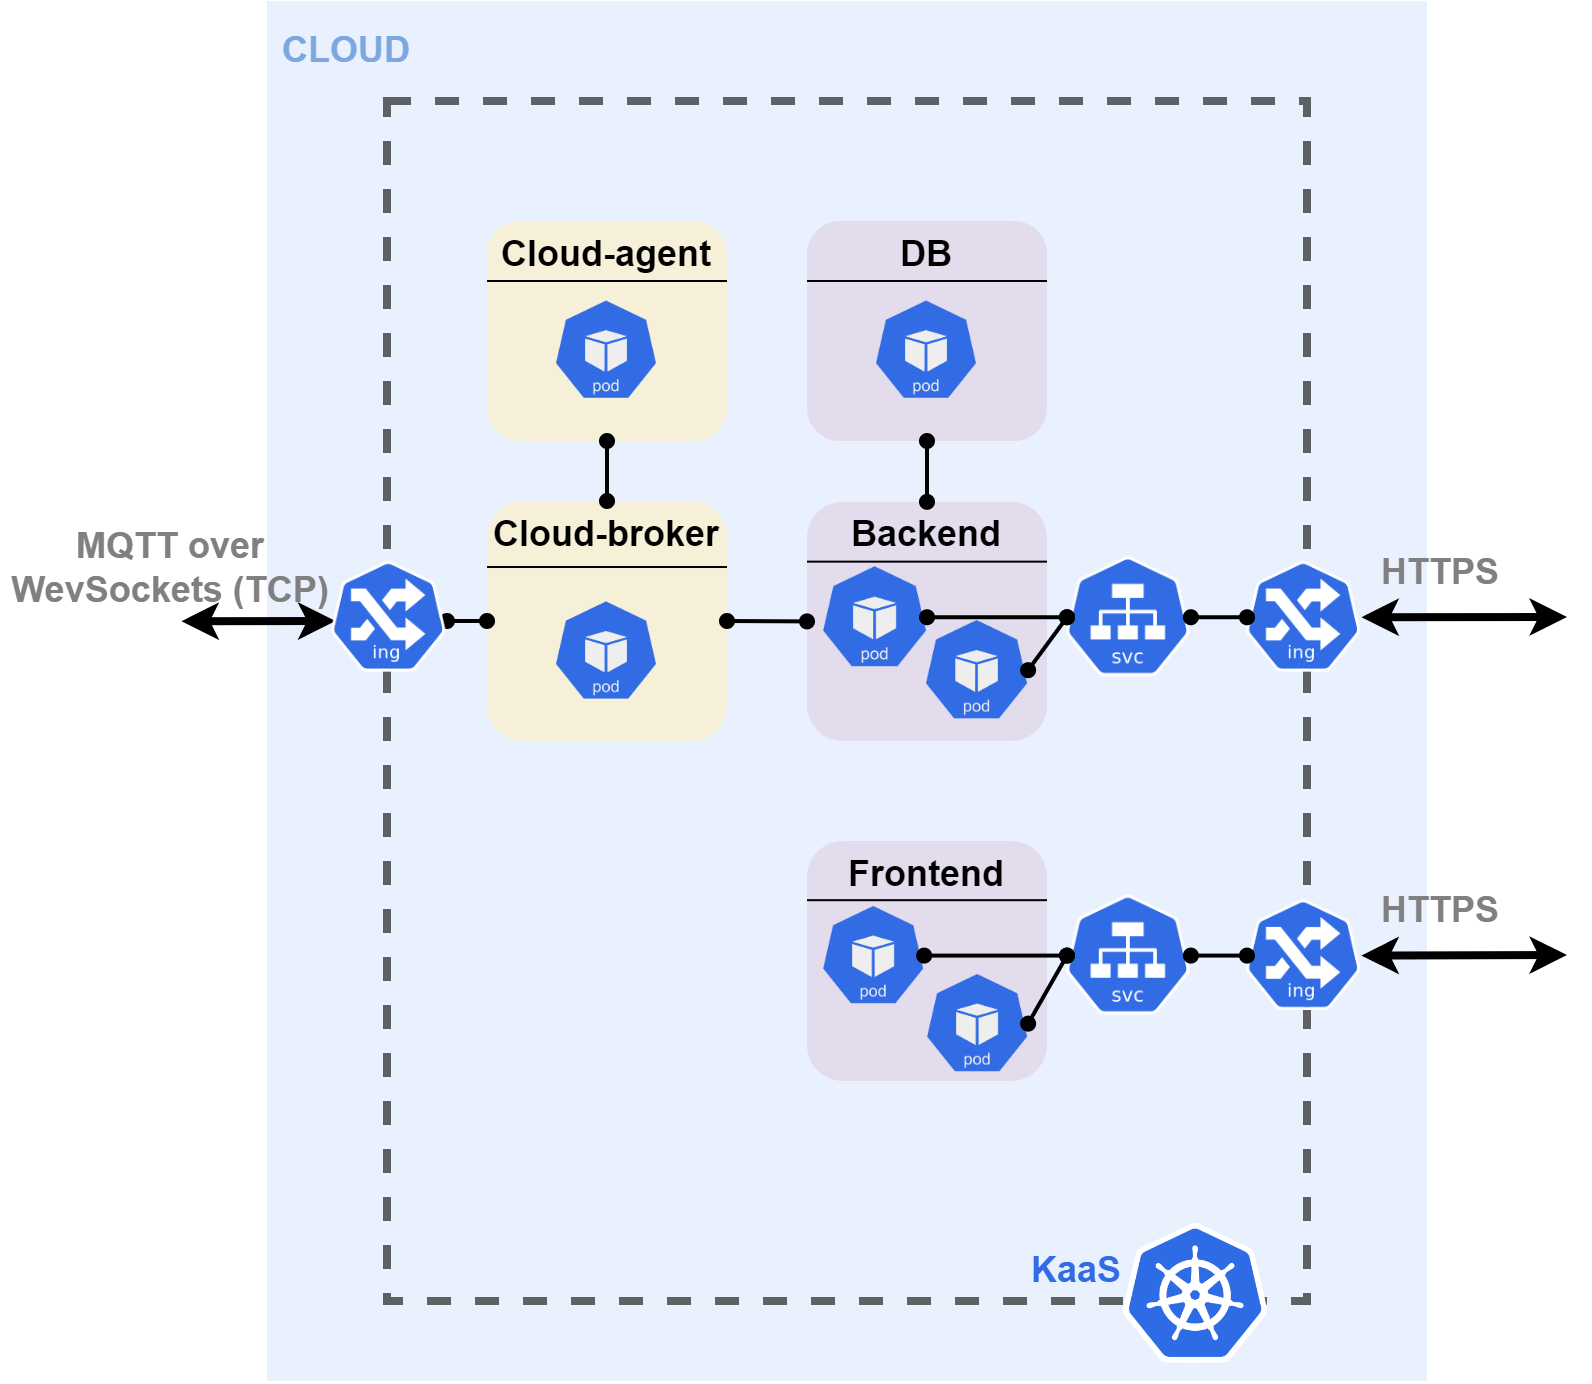
\includegraphics[width=0.85\textwidth]{pictures/cloud_services.png}
    \caption{Cloud services system design}
    \label{fig:cloud_services}
\end{figure}

In this system design, three endpoints are exposed to external traffic, which originates from outside of the cluster. These include two HTTP/HTTPS(Hypertext Transfer Protocol) endpoints for the Backend and Frontend and one WebSocket endpoint for MQTT messages that are sent to the cloud broker. HTTP/HTTPS traffic for frontend and backend is served through the use of ingress resources within the cluster. The traffic is forwarded via a reverse proxy (NGINX) to a Kubernetes service, which then distributes the request among the pods. The default ingress resource is designed to handle only HTTP/HTTPS requests and does not allow for any other protocol.

For the MQTT protocol, which is transported over TCP protocol, a NodePort \cite{kubernetes_docs} would typically be used to expose the service to the outside world. This maps pod ports to ports of the node in the cluster. However, some cloud providers do not permit the use of NodePorts, so a more flexible option was chosen, which involves bootstrapping the MQTT protocol over WebSockets and using ingress resources to handle external traffic coming to the cluster. This approach allows for the handling of MQTT traffic in a way that is compatible with the ingress resource and does not require the use of NodePorts.